\subsection{中文写作}
\begin{frame}{有关中文写作}
\begin{itemize}
    \item 宏包 \pkg{xeCJK}
    \item 参考 \url{https://www.overleaf.com/learn/latex/chinese}
\end{itemize}
\end{frame}

\begin{frame}[fragile]{中文示例}
  
    \begin{itemize}
        \item 编辑 \texttt{hello.tex} (Windows 下不要用中文文件名,注意
        \LaTeX{} 对文件名大小写敏感)
        \lstset{language=[LaTeX]TeX}
        \begin{lstlisting}[basicstyle=\ttfamily]
\documentclass{ctexart} % 使用中文适配的 article 文档类
\usepackage{xeCJK}%如果要在一般的文档内使用中文,一般只需引入此包
\begin{document}
\TeX{}你好!
\end{document}
          \end{lstlisting}
        \begin{itemize}
          \item Windows 下缺省使用中易字体
          \item Linux、macOS 下需要注意字体(参见 \pkg{ctex} 文档)
        \end{itemize}
      \item 使用 \XeLaTeX{} 引擎编译,得到 PDF 文档
        \begin{center}
          \fbox{\textrm \TeX{}\songti 你好!}
        \end{center}
    \end{itemize}
\end{frame}
  

\section{实践}
\subsection{论文排版}


\subsection{论文模板使用}
\begin{frame}[fragile]
  \frametitle{模板}
  \begin{itemize}
    \item<+-> 是什么?
  
      \begin{itemize}
        \item 设计好的格式框架
        \item 专注于内容:\alert{不要追求与期刊排版一致}
        \item Word 中的样式:「学好 \LaTeX{} 可以更科学地使用 Word」
      \end{itemize}
  
    \item<+-> 有哪些?
  
      \begin{itemize}
        \item 期刊:\pkg{revtex}、\pkg{elsarticle}、\pkg{IEEEtran}、\pkg{acmart}……
        \item 学位论文:\pkg{thuthesis}、\pkg{ustcthesis}、\alert{\pkg{sustechthesis}}……
      \end{itemize}
  
    \item<+-> 怎么用?
  
      \begin{itemize}
        \item |\documentclass{...}|,配置参数,照常编写
        \item \alert{看文档,看文档,看文档}
      \end{itemize}
  
    \item<+-> 去哪里找?
  
      \begin{itemize}
        \item CTAN \link{https://ctan.org} 或 GitHub \href{https://github.com}{\faGithub}
        \item 期刊/会议官网
        \item SUSTech LaTex 模板目录 \link{https://github.com/SUSTC/latex-template}
        \item 「U 盘拷给你的模板一定是过时的」
      \end{itemize}
  \end{itemize}
\end{frame}


\begin{frame}{论文排版}
    \begin{itemize}
      \item 获取模板
        \begin{itemize}
          \item 随发行版自带、手动官网下载
          \item 模板文档类 \texttt{.cls} 文件
          \item 示例 \texttt{.tex} 文件
        \end{itemize}
      \item 编辑 \texttt{.tex} 文件:添加用户内容
      \item 编译:生成 PDF 文档
    \end{itemize}
  \end{frame}
  
  \begin{frame}[fragile]{论文排版举例}
    \begin{exampleblock}{IEEE 期刊论文}
      \begin{itemize}
        \item 获取模板:已随发行版自带
          \begin{itemize}
            \item 在安装目录 |<prefix>\texlive\2020\texmf-dist\doc\latex\IEEEtran|
              下找到 |bare_jrnl.tex|
            \item 复制到某个文件夹(比如个人存论文的目录)
          \end{itemize}
        \item 编辑 |bare_jrnl.tex| 文件 (英文模板:不支持中文)
        \item 编译
          \begin{itemize}
            \item 英文文献:\XeLaTeX 、\pdfLaTeX 编译均可
          \end{itemize}
      \end{itemize}
    \end{exampleblock}
  \end{frame}



\subsection{作业与论文中的常用模板}
\begin{frame}{几种在作业/论文中常用的模版}
    \begin{columns}[c]
    \begin{column}{.45\textwidth}
        \begin{itemize}
            \item 毕业论文模版 \url{https://github.com/SUSTech-CRA/sustech-master-thesis}
            \item IEEE \url{https://template-selector.ieee.org/secure/templateSelector/publicationType}
            \item 同学制作的作业模板 \url{https://github.com/ziqin/LaTeX-SUSTechHomework}
        \end{itemize}
    \end{column}
    \begin{column}{.45\textwidth}
        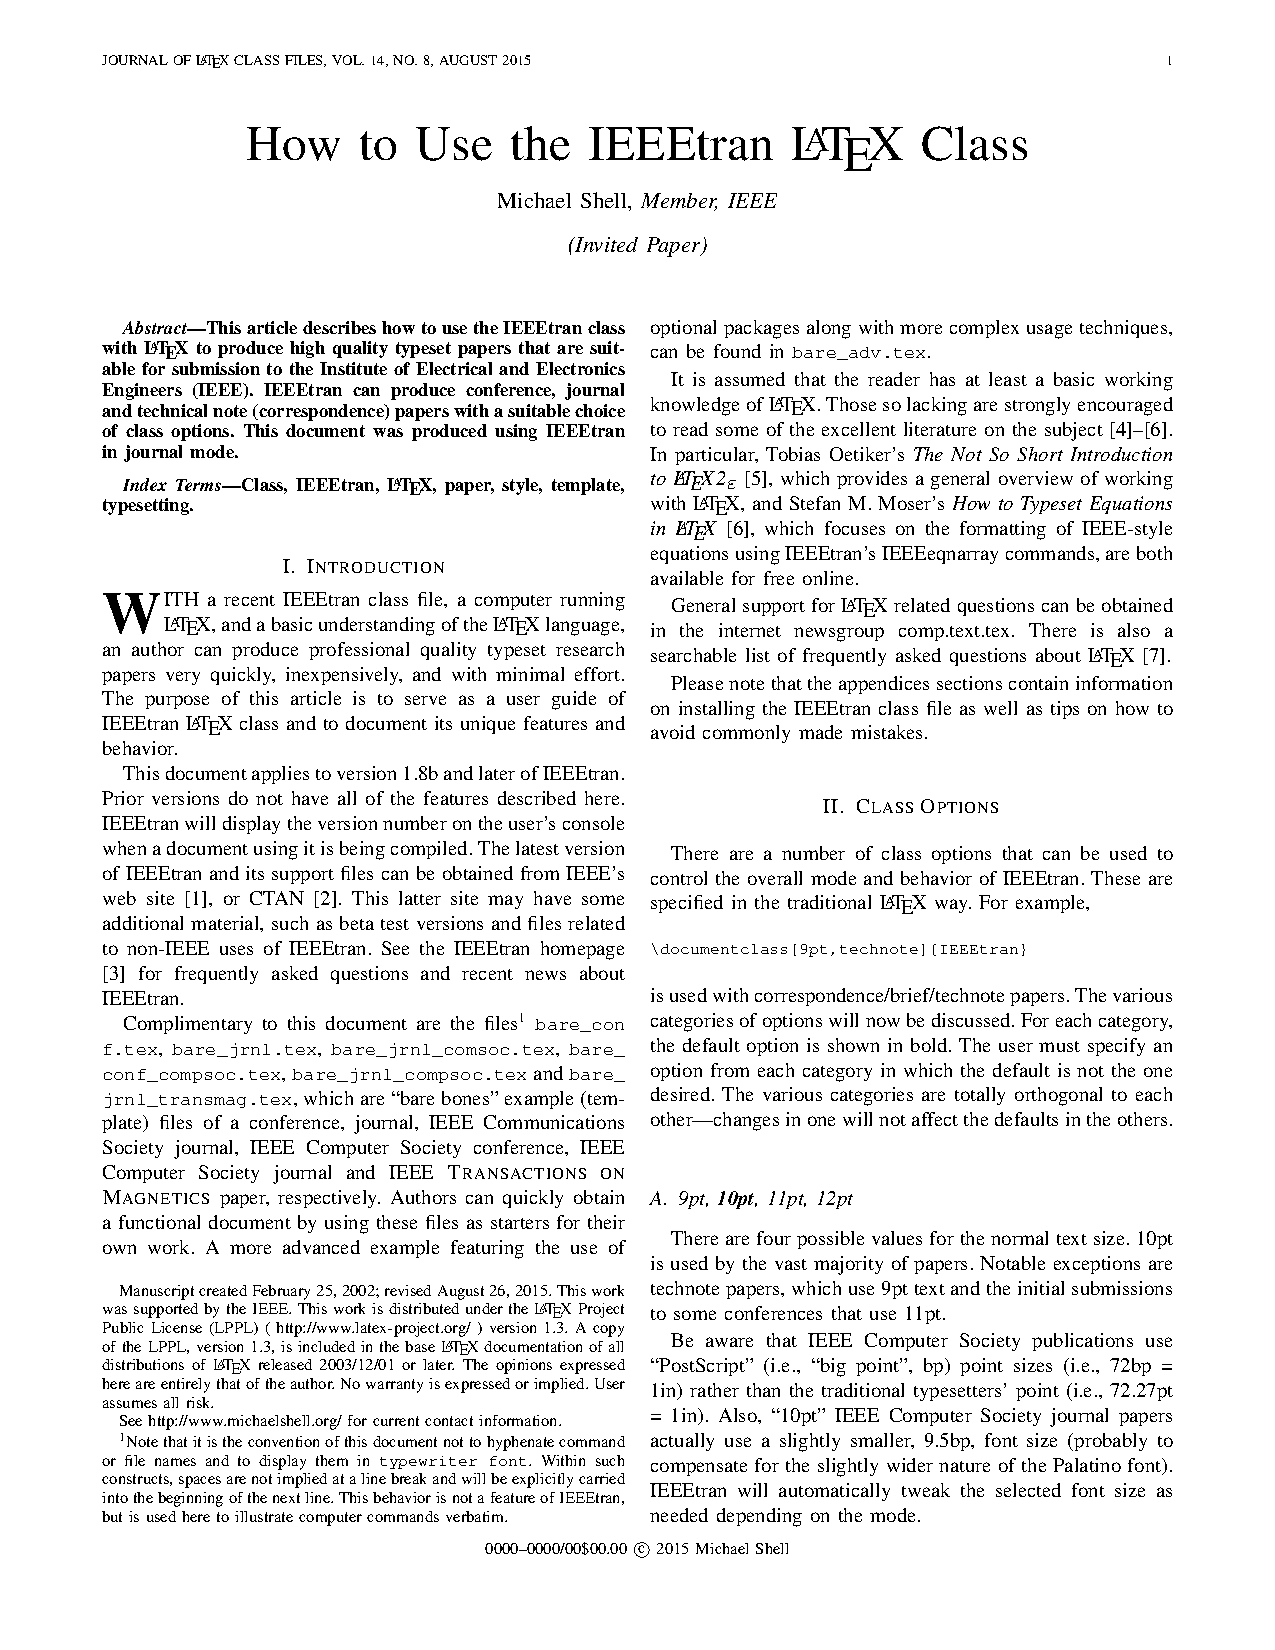
\includegraphics[width=0.75\textwidth]{docs/IEEE_template_1.pdf}
      \end{column}
    \end{columns}
    

\end{frame}
